\chapter{Force Estimation Algorithm}
\section{Estimation of Contact Force using Motor Torques}

After all necessary parameters have been identified, contact force can now be estimated using denso torques. The formula to measure the contact force is:

\begin{align}
\label{model eq}
  F_{contact} &= \left(J^{T}\right)^{-1} \left( K_{denso} \tau_{denso} -  \left( \tau_{dyn} + K_{c} sign\left(\dot{q}\right) + K_{v} \dot{q} \right))\\
  \tau_{dyn} &=M\left(q\right)\ddot{q} + C\left(\dot{q} , q \right)\dot{q} + G\left(q \right)
\end{align}

Where $ F_{contact} $ is the force that the robot gives to the object and $\tau_{dyn}$ is the torque due to the dynamic motion. Since dynamic model identification has not been performed, the calculation of $\tau_{dyn}$ could not be done manually and hence it relies on the result given from the OpenRave simulation. But before continuing further, the simulation result must be verified with the experimental data first to guarantee the truthness of the value. 

\section{Comparison of Denso Torque and OpenRave Simulation}
\label{Verification of Motor Torque Calibration}
To compare the value of calibrated denso torque with the OpenRave , a simple setup experiment can be done. The setup can be described like this: for one joint, the robot is positioned such that the motor will exert some torques due to the weight of the links only. Because it is not moving and no external force is introduced, the dynamic equation is reduced to be :

\begin{equation}
  K_{denso} \tau_{denso} = G\left(q \right) \\
\end{equation}

The value of $G\left(q \right)$ is computed using OpenRave. The value should be comparable to the left side of equation. 

\begin{figure}[H]
    \centering
    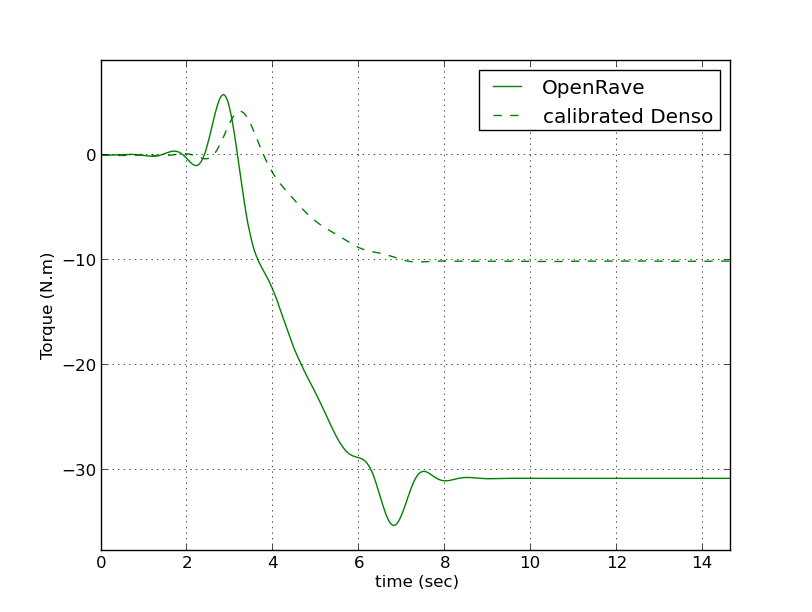
\includegraphics[width = 0.6\textwidth ]{high_tor_val}
    \caption{Joint Torque Verification for Second joint}
    \label{fig: tor verification}
\end{figure}

However, the figure in \fref{fig: tor verification} shows a different result. The continuous line represents the torque computed from OpenRave, (e.g.:$G\left(q \right)$) and the strip line represents the motor torque after calibration (e.g.: $K_{denso} \tau_{denso}$). It is very clear that values are not similiar. The value given in OpenRave is much higher than calibrated denso torque. There are two possibilites that might be the reason of this differences, which are: 1) The gain value ($ K_{denso} $) is incorrect due to some problems that might arise in F/T sensor (i.e.: F/T sensor not calibrated) or 2) The OpenRave gives incorrect computation. It is quite difficult to investigate the second reason as until now the real dynamic parameters of the Denso arm have not been identified, thus torque computation of dynamic motion could not be done for now except using OpenRave. On the other hand, the ATI F/T sensor should have been calibrated before the experiments, thus the first possibility is unlikey to happen. 

Hence, from this comparison it can be found that there are some pieces that are still missing. Since the OpenRave result has not been investigated whether it is truly correct or not, it is decided not to use the OpenRave to compute the dynamic torque. However, it makes a hole in the model estimation since the dynamic torque is required. To solve this problem, quasi-static assumption is used in the model to fill the hole in the model. 

\section{Quasistatic Based Model}

To solve the problem regarding $\tau_{dyn}$, the model is assumed to be quasistatic condition. It means that the changes of $\tau_{dyn}$ between pre-contact and contact is negligible and hence, it can be assumed to be constant. Thus by carefully selecting the pre-contact as a reference point, this term will dissappear in the equation (\ref{model eq}). Thus, the modified model equation becomes:

\begin{align}
\label{quasistatic}
  F_{contact} &= \left(J^{T}\right)^{-1} \left( K_{denso} \tau_{denso}^{\prime} -  \left(\tau_{fric} - \tau_{fric , ref}\right)\right)\\
  \tau_{fric} &= K_{c} sign\left(\dot{q}\right) + K_{v} \dot{q} 
\end{align}

Here $\tau_{denso}^{\prime}$ refers to the denso torque value after being referenced with the value during pre-contact position ($\tau_{denso}^{\prime} = \tau_{denso} - \tau_{denso , init}$) and $\tau_{fric , ref}$ is the friction at the pre-contact point. Since it relies on the assumption that $\tau_{dyn}$ is zero, there are two main limitations to this model. They are:

1) The pre-contact position cannot be too far from the contact point. 

2) The robot should not move and accelerate too fast since $\tau_{dyn}$ is very sensitive to these parameter.

Hence it is best to choose the reference point as close as possible to the contact area and move the robot slowly from there.

\section{Algorithm Flows}
\label{algorithm}

The following algorithm is created based on the quasistatic model that has been explained in the previous section. The steps of the algorithm are:

1) Move the robot to the pre-contact position. It is preferred to choose the point as close as possible to the contact area.

2) Move the robot slowly to the contact position.

3) Quickly make the initialization to the denso torque and friction. For each joint, take the current value of the denso torque as a zero-based value ($\tau_{denso , init} $) and calculate the friction from the joint velocity and store the value in the $\tau_{fric , ref}$. There are two points that can be choosen as reference points, they are: A. The point where the robot is not moving yet (step 1) or B. The point right after the robot starts to move (step 2). The only difference about these twp points is about the presence of friction. However, since the friction has been identified, ideally these two points should give the same results.

4) Estimate the contact force based on denso torques and joint velocities. The denso torque is then subtracted by $\tau_{denso , init}$ to get $\tau_{denso}^{\prime}$ while joint velocity is used to estimate the friction part. Use the equation (\ref{quasistatic}) to get the contact force estimation.

These steps are the general steps required to compute the contact force. Some adjustments can be added accordingly depending on the usage of the algorithm (i.e.: whether it is used for offline computation or real time computation). The snippet code for the developed algorithm is available in the appendix (see \fref{fig:algo code}). The codes are developed in Python language.
